\begin{landscape}
\begin{figure*}[!htbp]
    \centering
    \begin{subfigure}[t]{0.625\textwidth}
        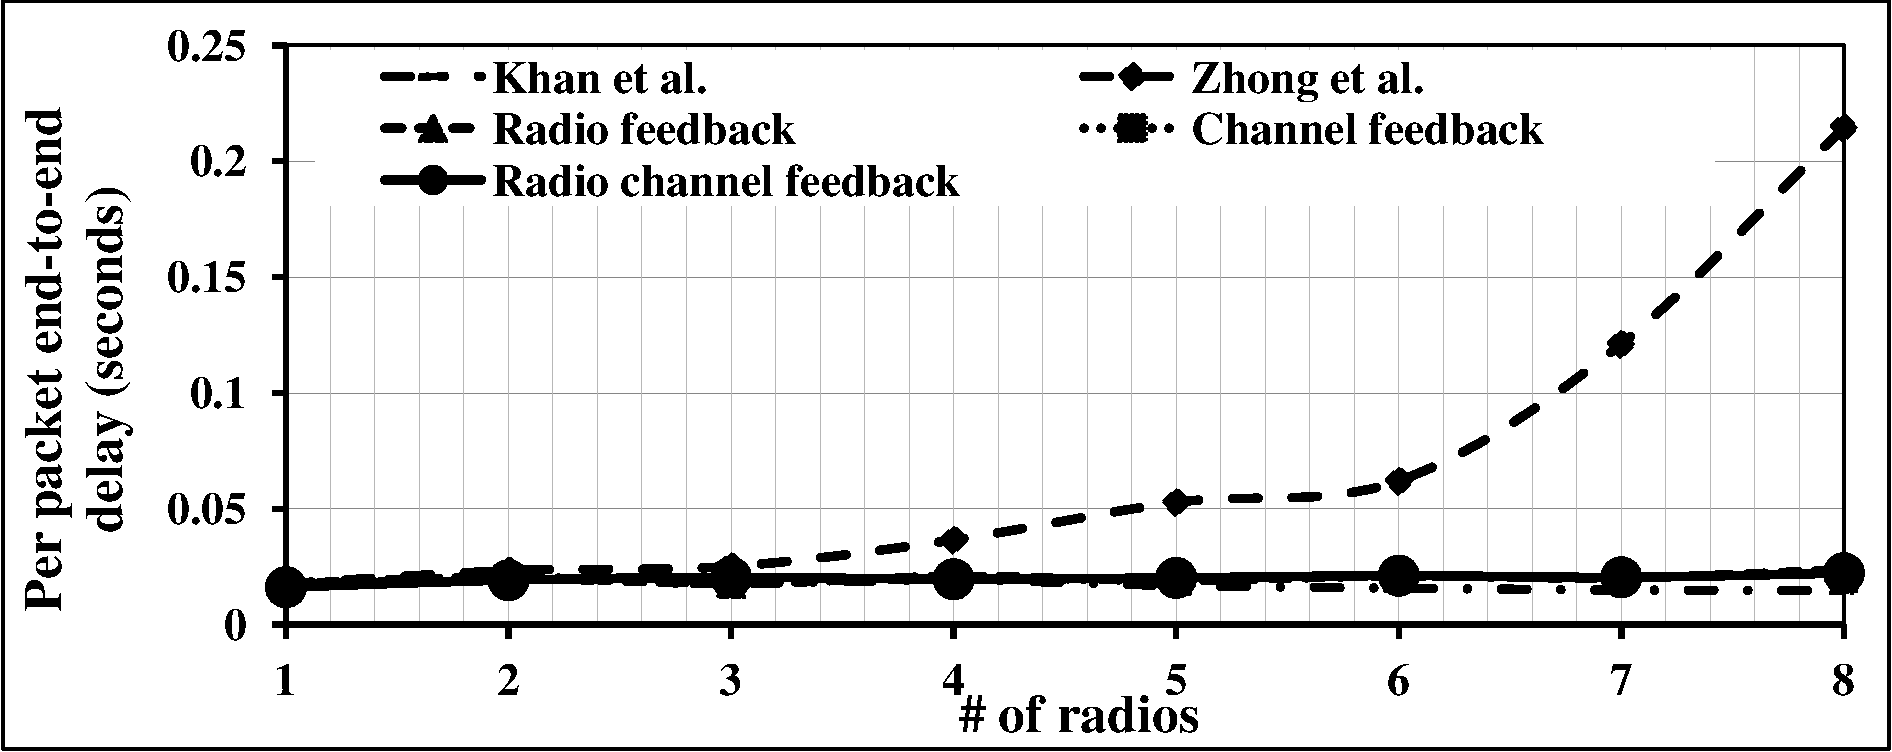
\includegraphics[width=\textwidth]{topology4/Delay24d1}
        \caption{1Mbps application data rate}
        \label{fig:topology4D1}
    \end{subfigure}
    ~
    \begin{subfigure}[t]{0.625\textwidth}
        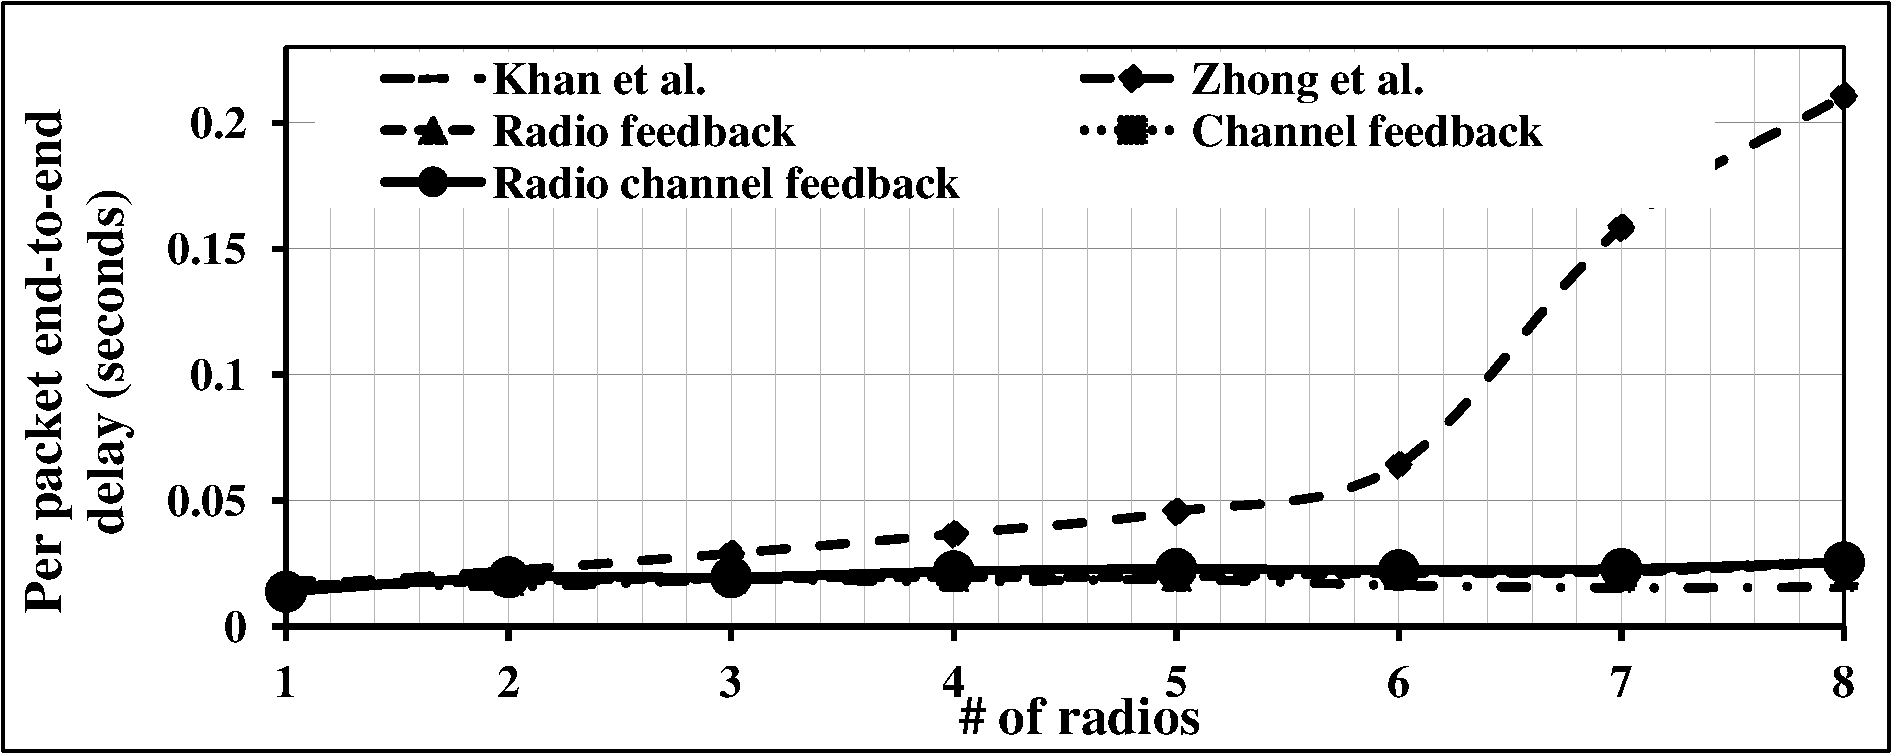
\includegraphics[width=\textwidth]{topology4/Delay24d2}
        \caption{2Mbps application data rate}
        \label{fig:topology4D2}
    \end{subfigure}
    ~\\
    \begin{subfigure}[t]{0.625\textwidth}
        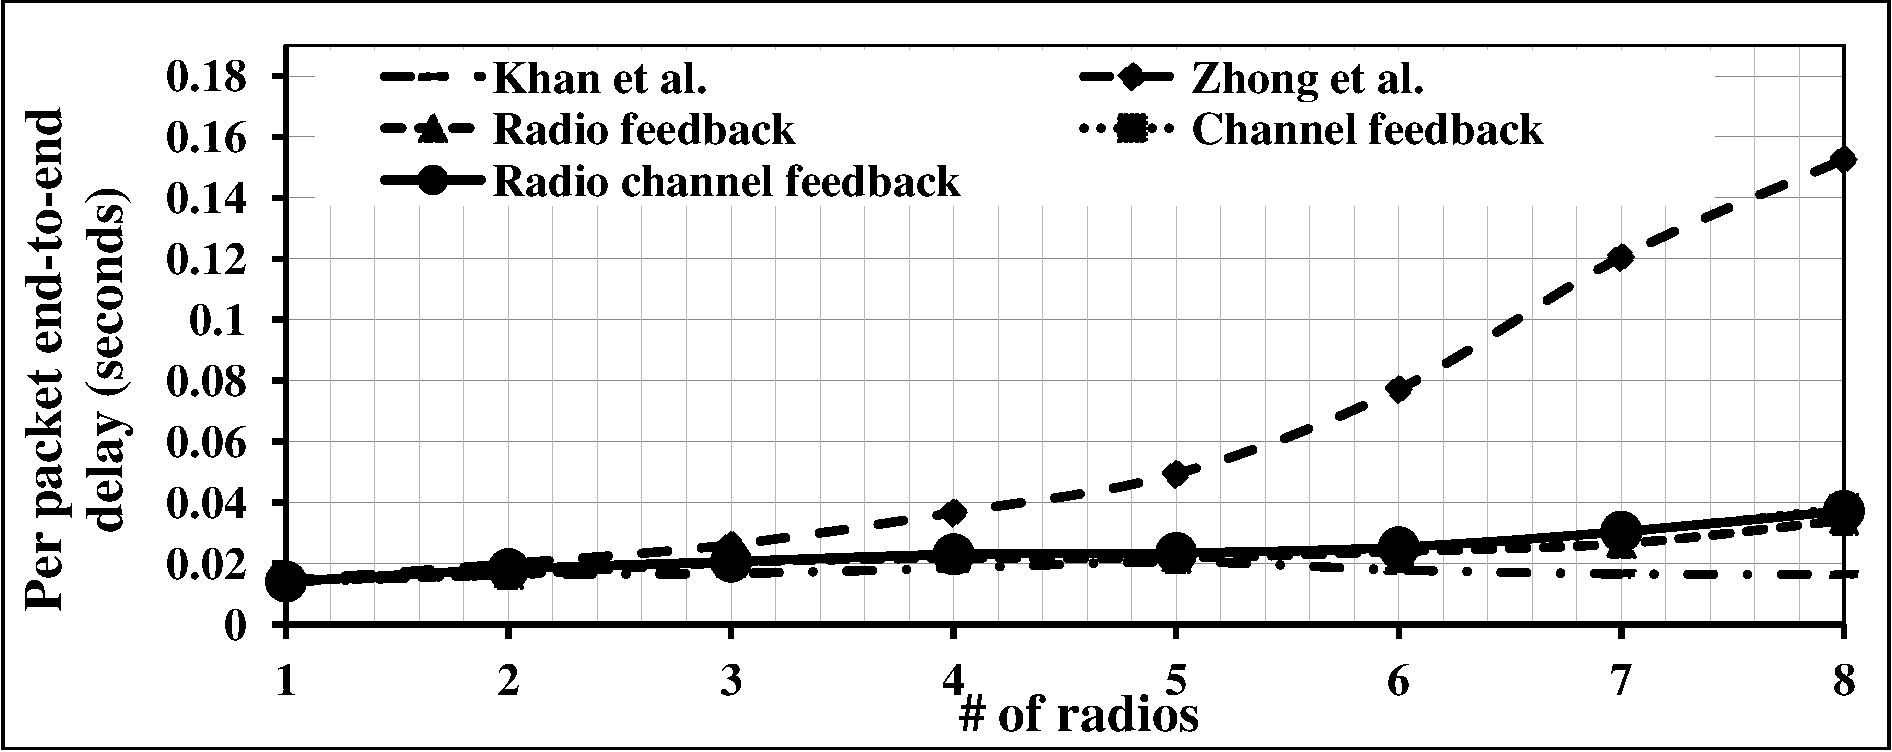
\includegraphics[width=\textwidth]{topology4/Delay24d4}
        \caption{4Mbps application data rate}
        \label{fig:topology4D3}
    \end{subfigure}
    ~
    \begin{subfigure}[t]{0.625\textwidth}
        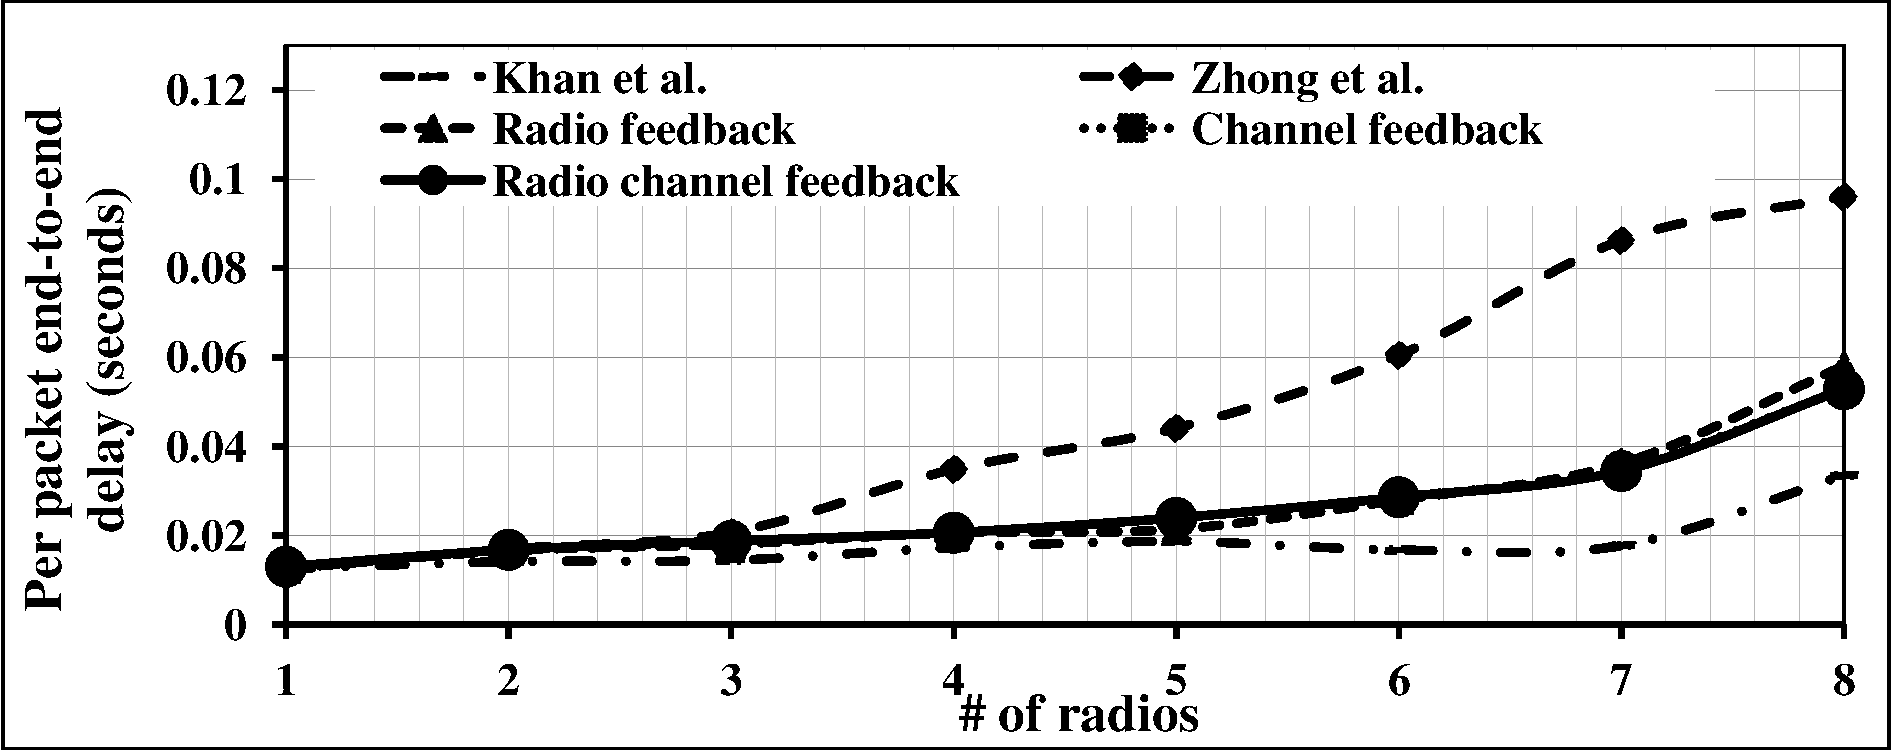
\includegraphics[width=\textwidth]{topology4/Delay24d8}
        \caption{8Mbps application data rate}
        \label{fig:topology4D4}
    \end{subfigure}
    ~\\
    \begin{subfigure}[t]{0.625\textwidth}
        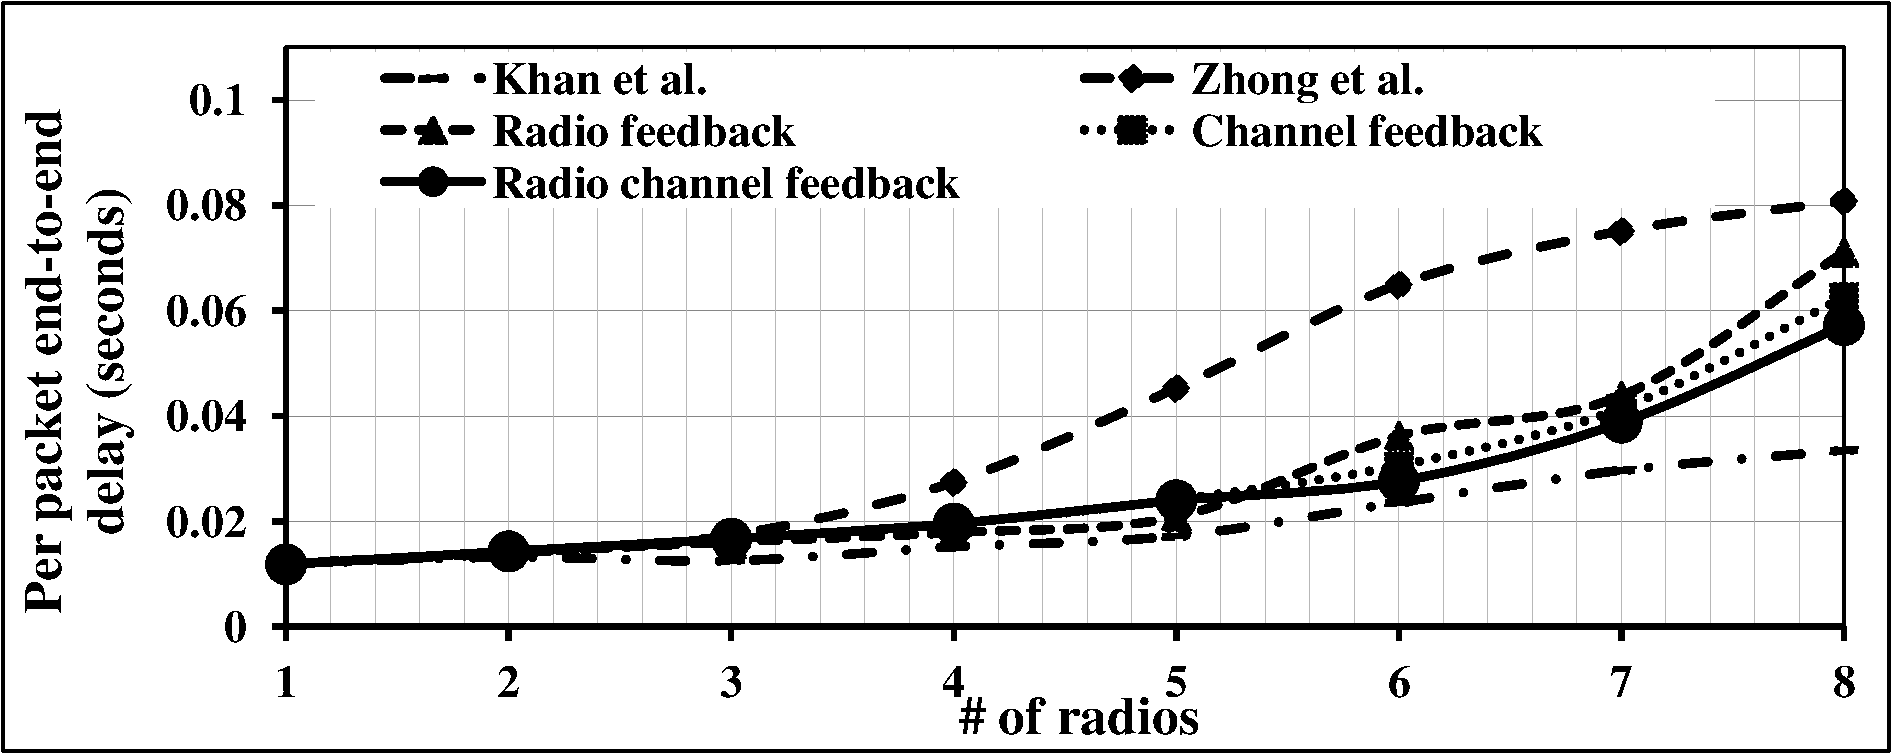
\includegraphics[width=\textwidth]{topology4/Delay24d16}
        \caption{16Mbps application data rate}
        \label{fig:topology4D5}
    \end{subfigure}
    ~
    \begin{subfigure}[t]{0.625\textwidth}
        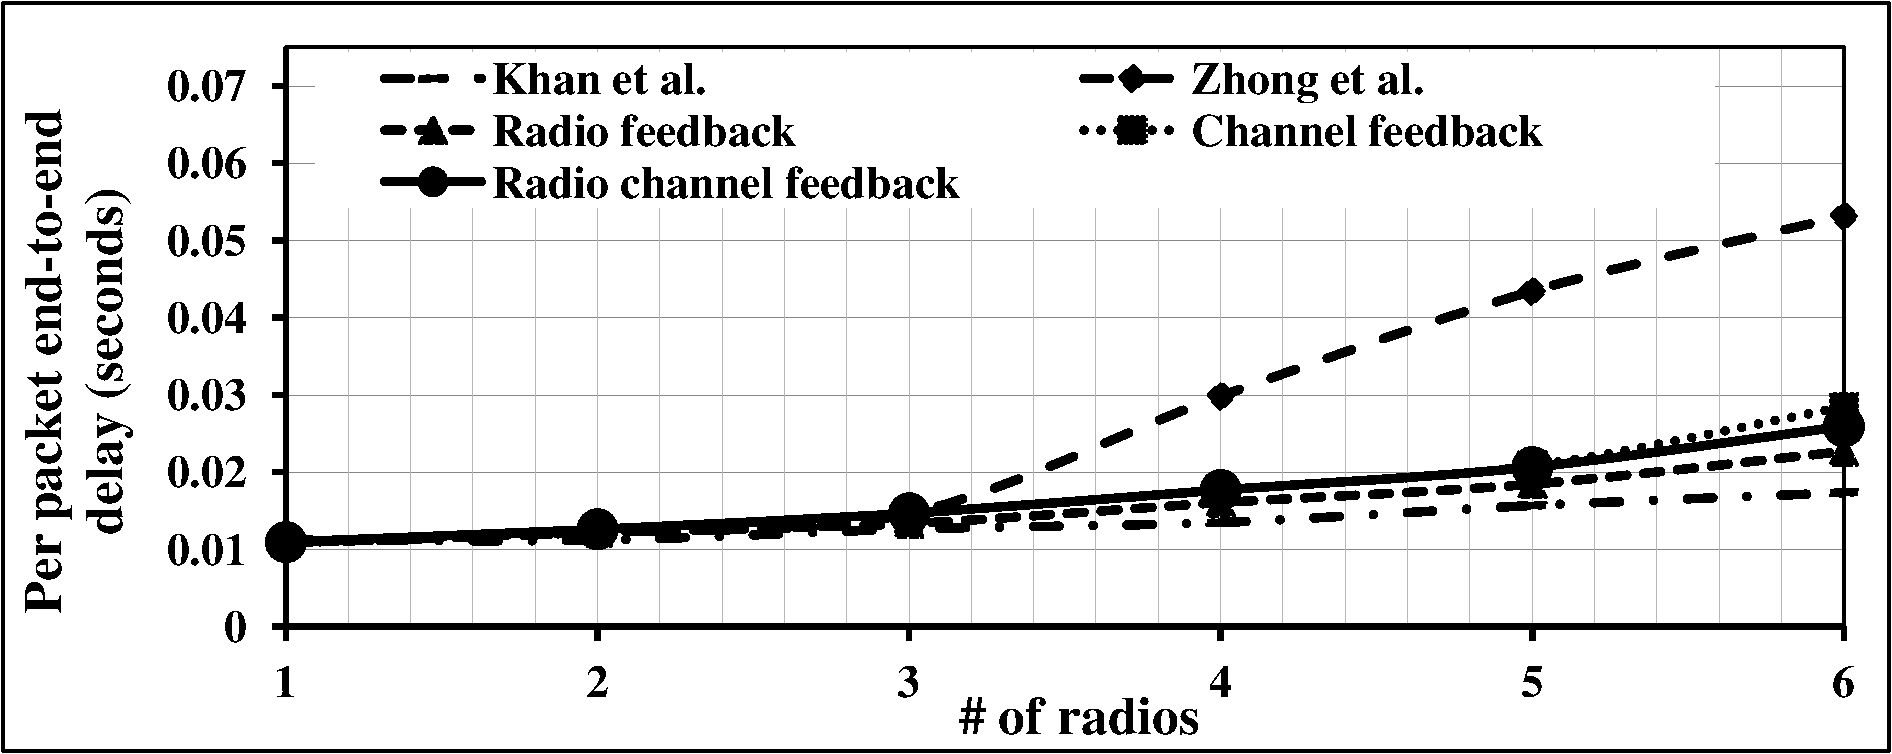
\includegraphics[width=\textwidth]{topology4/Delay24d32}
        \caption{32Mbps application data rate}
        \label{fig:topology4D6}
    \end{subfigure}
    \caption{Average end-to-end delay with varying number of radios for various application data rates}
    \label{fig:topology4D}
\end{figure*}
\end{landscape}
